Els experiments per validar la implementació de l'algorisme han estat limitats
per diferents factors. En primer lloc, ha estat difícil aconseguir una bona
validació del funcionament de l'algorisme en Simulink perquè les simulacions
són bastant lentes, degut a que Vitis Model Composer imposa un període
del solver igual o inferior al període de rellotge escollit. Una solució
possible és realitzar un model del motor en FPGA a mode de \emph{hardware in
the loop}. Malauradament, es decidí no implementar aquest experiment en l'abast
d'aquest projecte i provar d'implementar el control directament sobre la FPGA i
realitzar les proves directament amb les plaques de potència, cosa que
finalment no s'ha aconseguit.

\subsection { Test unitaris }
{
    S'han realitzat una sèrie de tests unitaris de diversos components de
    l'algorisme per testejar el seu funcionament.

    \paragraph{Sinus i cosinus} S'introdueix un senyal dent de serra a
        l'entrada del subsistema i es compara el resultat amb un bloc de
        generació de sinus i cosinus nadiu de Simulink. La freqüència del
        senyal a l'estrada és molt major a la que s'emprarà en realitat; però,
        ens permet fer-nos una idea del retard (delay) de l'operació i de la
        resolució temporal, en el nostre cas dos vegades el periode de rellotge
        del sistema.

        \begin{figure}[!htb]
            \centering
            \captionsetup{justification=centering,margin=1.5cm}
            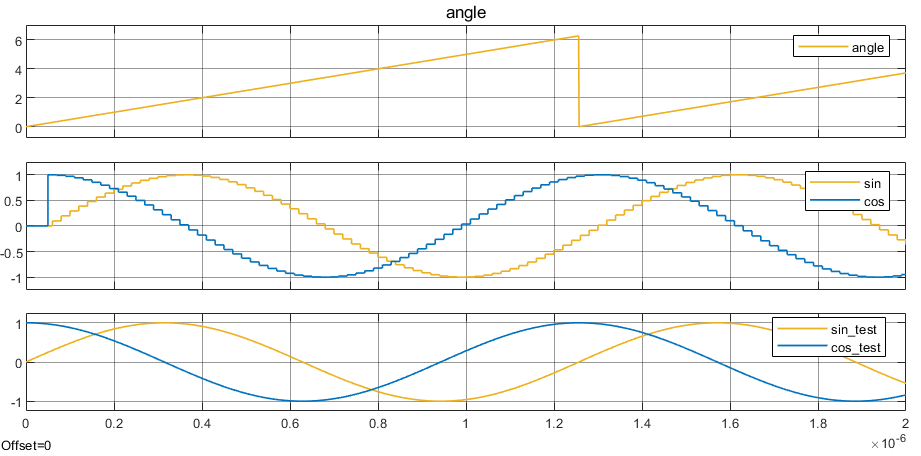
\includegraphics[width=8cm]
                {img/5_resultats/sineLUT_test.png}
            \caption{ Prova de la implementació del sinus i del cosinus }
        \end{figure}
    

    \paragraph{Senyal triangular} Es pot veure en aquest test que senyal
        triangular del PWM es genera a la freqüència correcta i l'amplitud en
        coma fixa s'intrpreta correctament.
    
        \begin{figure}[!htb]
            \centering
            \captionsetup{justification=centering,margin=1.5cm}
            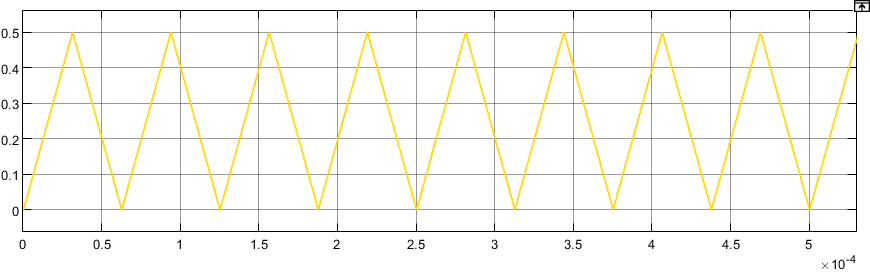
\includegraphics[width=8cm]
                {img/5_resultats/triangular.png}
            \caption{ Prova de la implementació del senyal triangular pel PWM }
        \end{figure}     
    

    \paragraph{SVPWM} Per a la prova del SVPWM, s'introduix com entrada dos
        senyals sinusoidals desfasats 90º. Simulem així un vector espacial de
        magnitud i frqüència de rotació constant i obtenim la forma d'ona
        característica de l'SVPWM.

        \begin{figure}[!htb]
            \begin{minipage}[c]{7.5cm}
                \centering
                \captionsetup{justification=centering}
                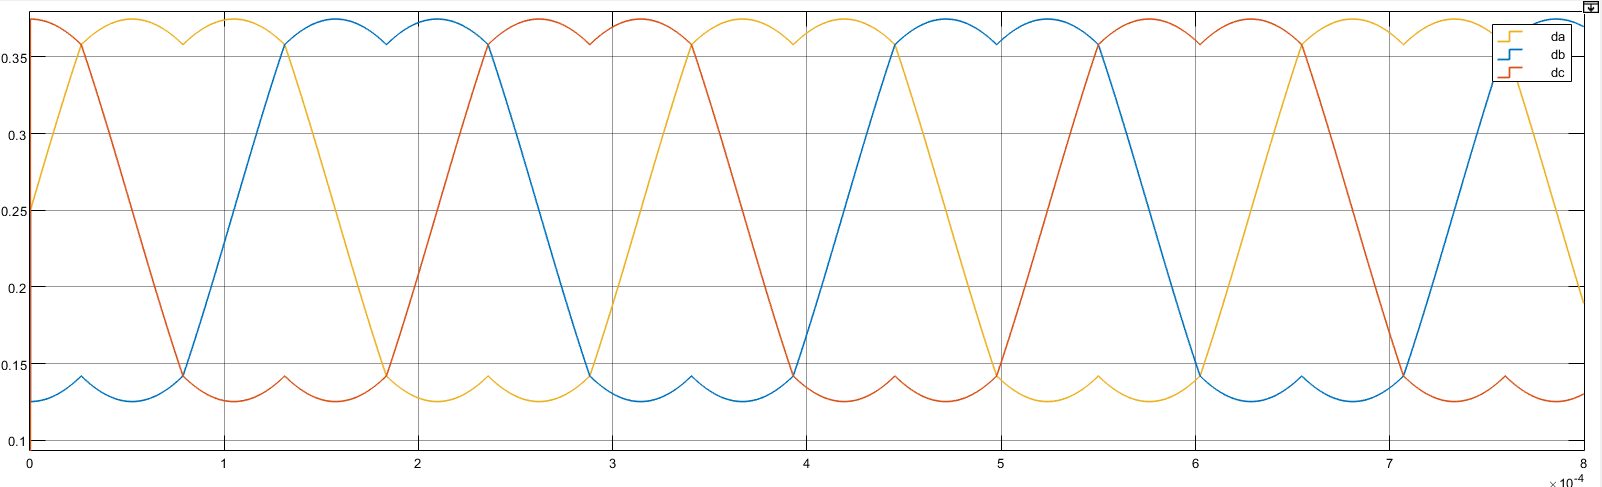
\includegraphics[width=7cm]
                    {img/5_resultats/sv_test.png}             
            \end{minipage} \hfil \hfil
            \begin{minipage}[c]{7.5cm}
                \centering
                \captionsetup{justification=centering}
                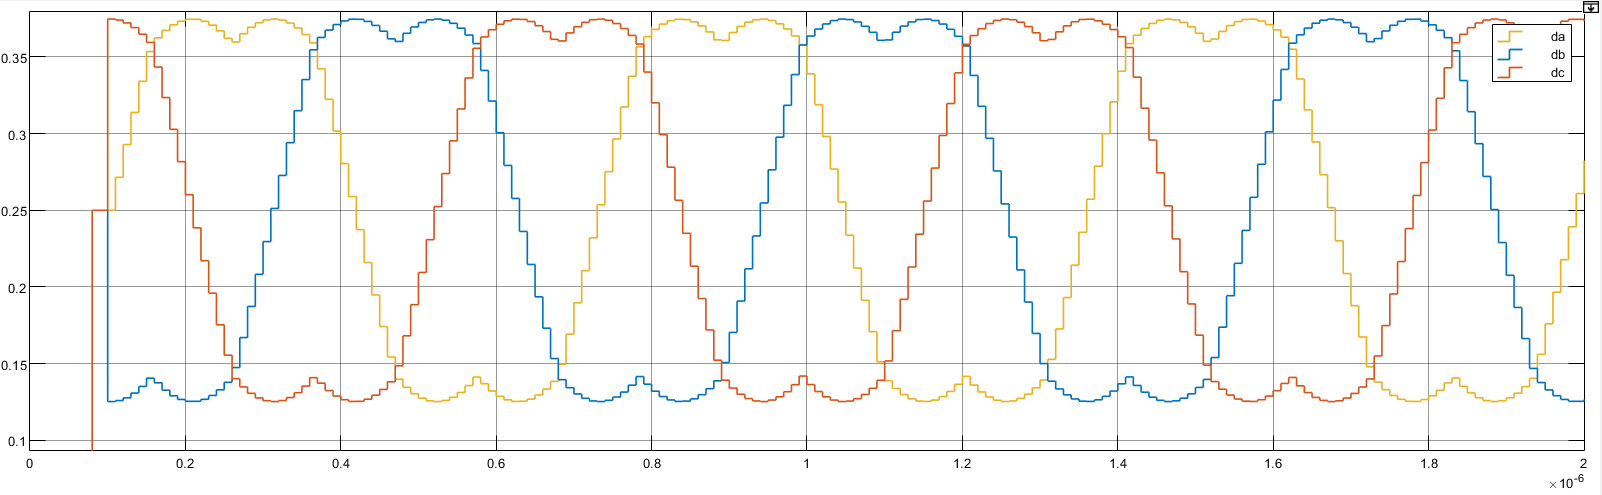
\includegraphics[width=7cm]
                    {img/5_resultats/sv_test2.png}           
            \end{minipage} \hfil
            \caption[Proves d'implementació de l'SVPWM]
            {  
                Proves d'implementació de l'SVPWM. A la dreta la 
                freqüència del senyal s'apropa molt més a la freqüència de
                rellotge del sistema.
            }
        \end{figure} 
        
    \paragraph{Limitador de voltatge} S'excita el bloc amb un senyal en rampa
        de $v_d$ i $v_q$ i s'observa que es limita el voltatge quan la magnitud
        del vector $v$ supera els $\frac{V_{DC}}{\sqrt{3}}$.
    
        \begin{figure}[!htb]
            \centering
            \captionsetup{justification=centering,margin=1.5cm}
            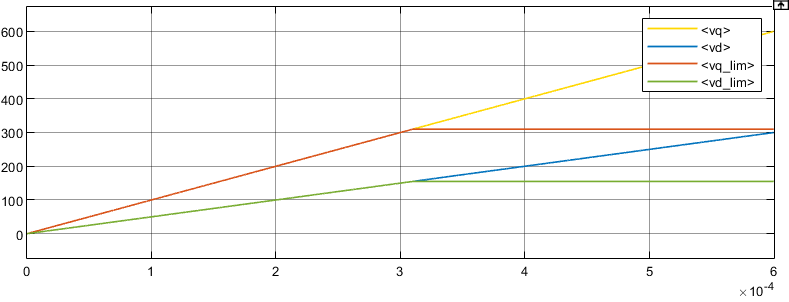
\includegraphics[width=7.5cm]
                {img/5_resultats/limitador.png}
            \caption{ Prova de la implementació del limitador de voltatge }
        \end{figure}     
    
}

\subsection{Simulacions de l'algorisme complet}
{
    En aquest subapartat s'analitzen les prestacions de l'algorisme de control
    implementat en el seu conjunt. Per provar la implementació realitzada es
    substitueix l'algorisme en el model de Simulink desenvolupat per l'equip.
    El model de l'inversor és el commutat i el model de l'inversor s'implementa
    a partir de les equacions del motor en el sistema de referència $d\-q$. És
    per això que s'implementen la transformada i la transformada inversa
    de Park a l'interior del subsistema del motor. 

    \begin{figure}[!htb]
        \centering
        \captionsetup{justification=centering,margin=1cm}
        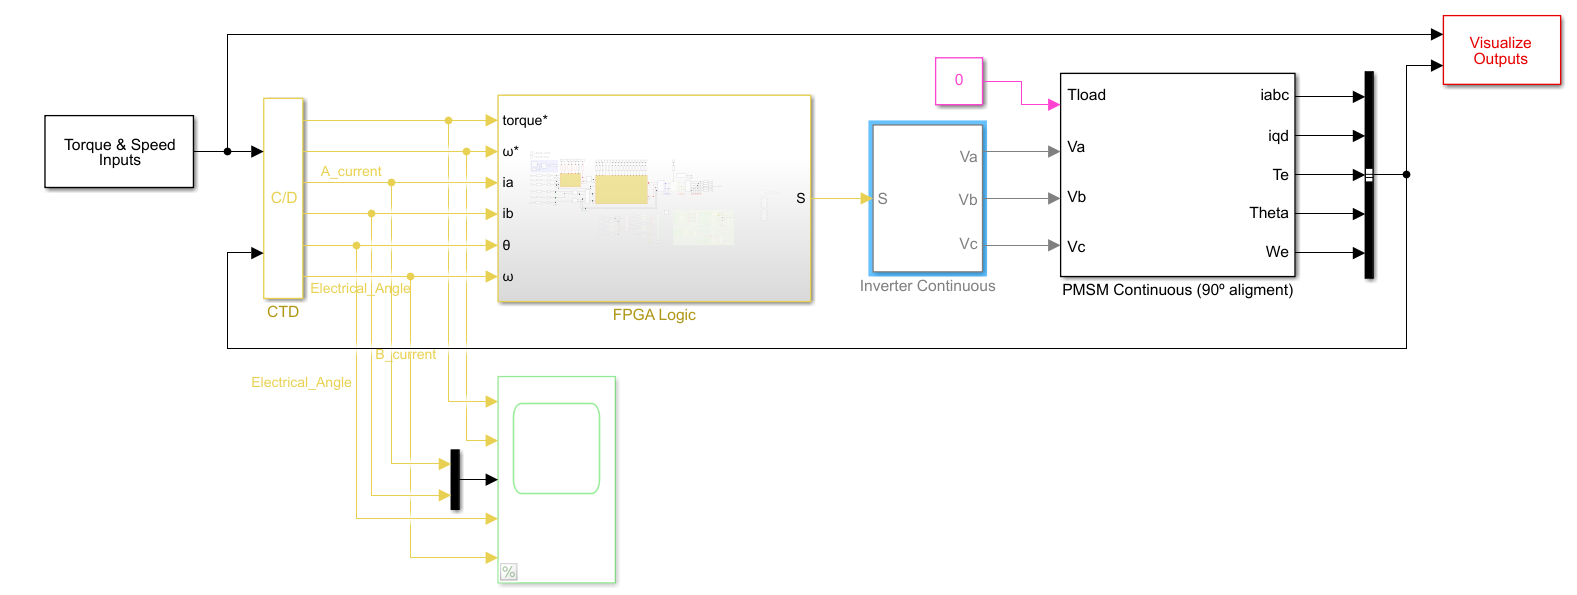
\includegraphics[width=11cm]
            {img/5_resultats/control.png}
        \caption[Model de Simulink desenvolupat per l'equip]{ Model de Simulink desenvolupat per l'equip, on el bloc de control ha set substituit per la implementació en FPGA. }
    \end{figure}

    \subsubsection{ Resultats de la simulació }
    {
        Si realitzem una simulació de la implementació del control en Simulink,
        podem veure com obtenim una rotació accelerada del rotor.

        \begin{figure}[!htb]
            \centering
            \captionsetup{justification=centering,margin=1.5cm}
            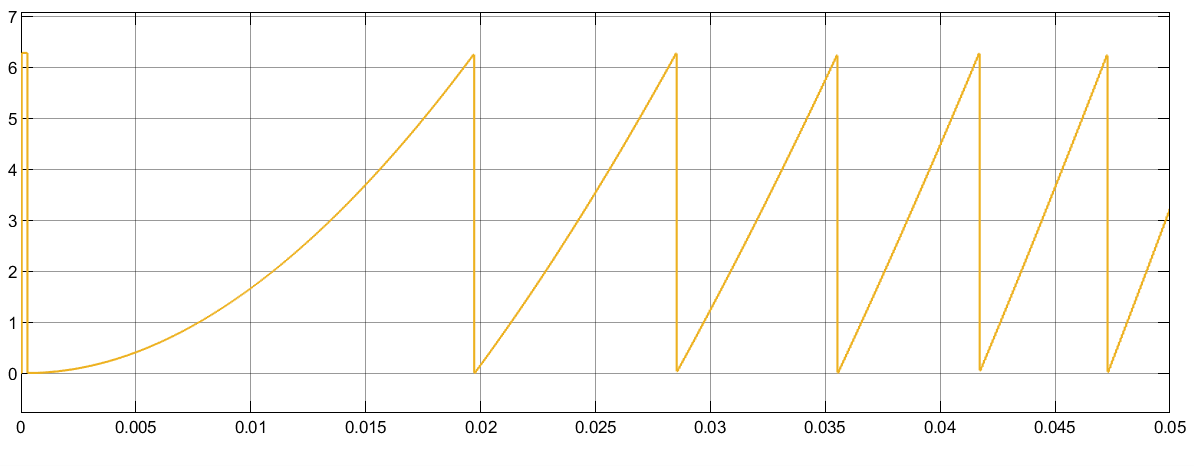
\includegraphics[width=6cm]
                {img/5_resultats/angle.png}
            \caption{ Angle del rotor respecte l'estàtor. }
        \end{figure}

        Per accelerar lleugerament la simulació, feim una decimació dels
        punts emmagatzemats per Simulink. Obtenim els resultats següents:
        
        \begin{figure}[!htb]
            \centering
            \captionsetup{justification=centering,margin=1.5cm}
            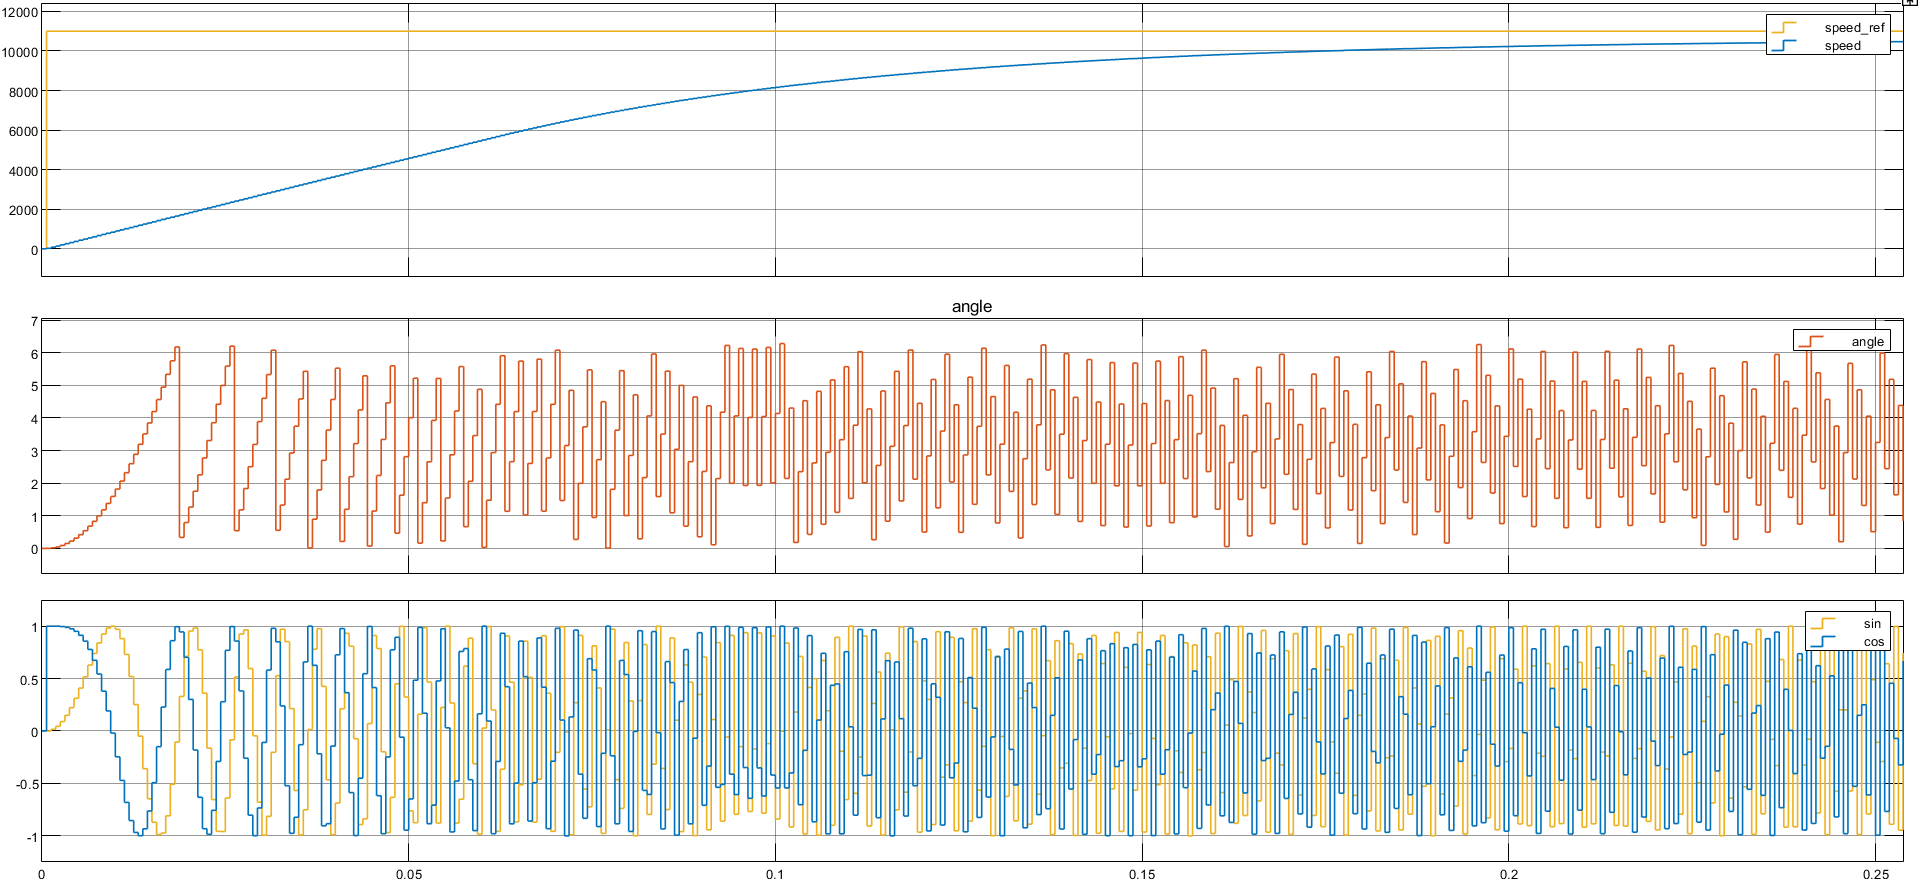
\includegraphics[width=10cm]
                {img/5_resultats/test.png}
            \caption[Resultat de la simulació (I)]{
                Resultat de la simulació. A dalt hi tenim la referència de
                velocitat i la velocitat real. Enmig tenim l'evolució de l'angle
                amb el temps. Abaix tenim l'evolució del sinus i del cosinus de
                l'angle.
            }
        \end{figure}

        \begin{figure}[!htb]
            \centering
            \captionsetup{justification=centering,margin=1.5cm}
            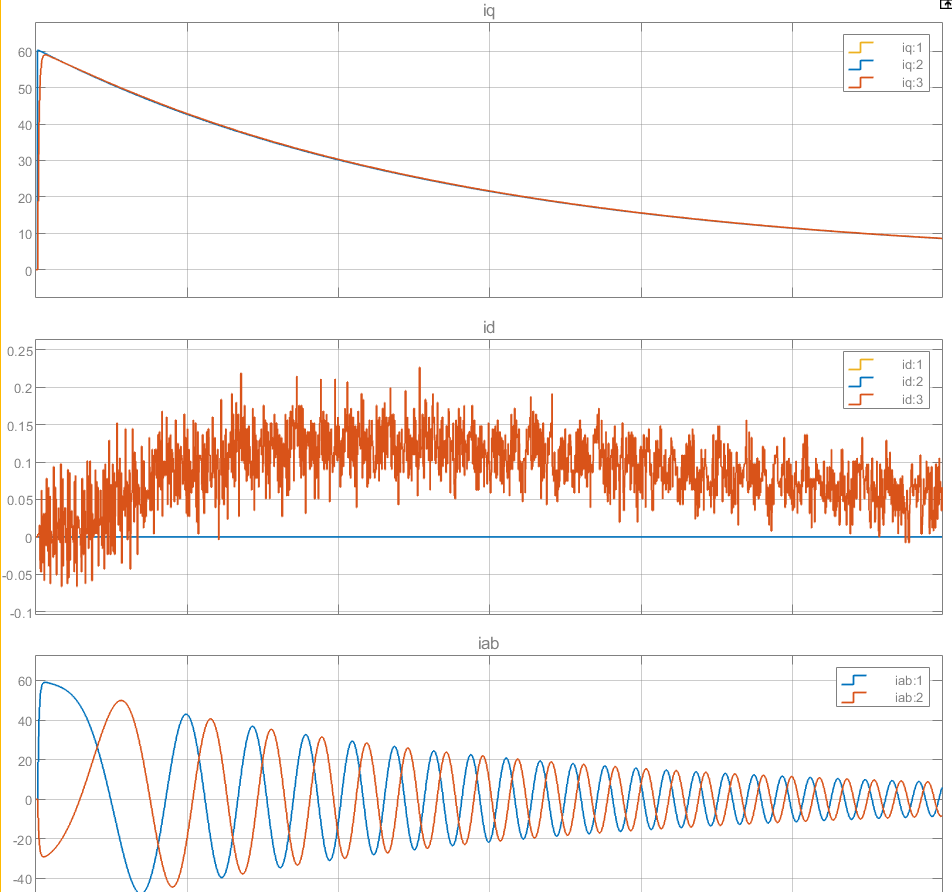
\includegraphics[width=8cm, height=5cm]
                {img/5_resultats/Untitled.png}
            \caption[Resultat de la simulació (II)]{
                Resultat de la simulació. A dalt hi tenim la referència de
                corrent $i_q*$ i el corrent $i_q$; just a sota el mateix pel
                corrent $i_d$. Abaix tenim l'evolució dels corrents $i_a$ i $i_b$
                (marc de referència de l'estator).
            }
        \end{figure}
    }
}